\documentclass{article}
\usepackage[spanish]{babel}
\usepackage[utf8]{inputenc}
\usepackage[nonatbib]{../template}

\usepackage[utf8]{inputenc} % allow utf-8 input
\usepackage[T1]{fontenc}    % use 8-bit T1 fonts
\usepackage{hyperref}       % hyperlinks
\usepackage{url}            % simple URL typesetting
\usepackage{booktabs}       % professional-quality tables
\usepackage{amsfonts}       % blackboard math symbols
\usepackage{nicefrac}       % compact symbols for 1/2, etc.
\usepackage{microtype}      % microtypography
\usepackage{xcolor}         % colors
\usepackage{graphicx}
\usepackage{float}
\usepackage[backend=biber,sorting=ynt,style=apa]{biblatex}

\addbibresource{../bibliography.bib}

\graphicspath{ {../imagenes/} }

\title{Entrega 3: Introducción y Resultados}

\author{José Saint Germain \texttt{josesg998@gmail.com} }

\begin{document}

\maketitle

% add TOC
\pagebreak
\tableofcontents
\pagebreak

\section{Introducción}

% Explicar la merma de golpes de estado, en especial en LATAM

% Mencionar dos o tres autores que mencionen los motivadores de golpes

El objetivo de este trabajo es lograr entrenar un modelo de aprendizaje automático
que logre predecir de manera aceptable la presencia de golpes de estado durante los años 
2020 a 2022 en todos los países del mundo a partir de la utilización de la base de datos 
provista por la fundación Varieties of Democracy (V-Dem) (\cite{Cop24}), 
así como tener una noción acabada de las variables más importantes que los algoritmos 
utilizan para la predicción de la variable objetivo.

\subsection{Motivación}
% Motivación del paper (comparar con el poder predictivo de la base del FMI)
La motivación de este trabajo es dialogar con el artículo recientemente realizado por el 
Fondo Monetario Internacionl (FMI) \cite{Ceb24}. En el mismo se aborda el mismo objeto 
de estudio utilizando diversas metodologías, siendo una de ellas la utilización de 
algoritmos de aprendizaje automático. En este trabajo se replicó la metodología utilizada 
en esa sección; comparando los mismos modelos, sus respectivos hiperparámetros y la 
métrica a maximizar durante su entrenamiento

La principal diferencia entre el paper del organismo y este trabajo radica en el origen
de los datos. Por un lado, el artículo del FMI utilizan 14 fuentes provenientes de 
diferentes organismos, de manera de cubrir 5 grupos de variables sobre diferentes ámbitos 
(Desarrollo y demografía, Inclusión y gobernanza, macroestabilidad, políticas públicas, 
estabilidad sociopolítica). En cambio, este trabajo utilizará solamente la base de datos 
v-dem por dos motivos: en primer lugar, para abarcar solamente variables que estén 
directamente ligadas a la situación política e insitucional de los países, excluyendo en 
la medida de lo posible atributos ajenos a este ámbito. En segundo lugar, para realizar 
una comparación con las nutridas y variadas fuentes del artículo citado. De esa manera, 
podemos tener una noción del poder predictivo de atributos puramente 
político-institucionales frente a un abanico más diverso de variables.

\subsection{Estructura del documento}
- Explicación de la estructura del trabajo (se realizará una vez que esté completado)

% limitaciones TODO

\section{Marco Teórico y estado del arte}

El estudio de los golpes de estado, así como los procesos de democratización han sido una 
preocupación central para la ciencia política moderna durante el siglo xx. Diversas teorías
y contrateorías se han desarrollado de manera de aprehender los causales de la democratización
de un país así como de su proceso inverso, ya sea una erosión democrática gradual o un
golpe de estado autoritario; así como los elementos sociales, culturales e institucionales 
que pueden evitar o disminuir la probabilidad de que se produzcan estos fenómenos.

\subsection{La Teoría de la Modernización y sus variantes}

Uno de los primeros marcos para comprender la inestabilidad política que llevaba a un golpe
institucional fue la teoría de la modernización, popularizada a mediados del siglo xx. 
Entre los exponentes de esta teoría se
encuentra Seymour Martin Lipset quien con su artículo \textit{"Some social requisites 
of democracy: economic developmente and political legitimacy"} (\citeyear{lipset1959some}). 
Desde un enfoque sociológico, 
argumenta que el grado de desarrollo económico de una sociedad es una condición 
necesaria para el nacimiento y consolidación de un régimen democrático, principalmente
porque una sociedad dividida entre una masa empobrecida y una élite rica es más
propensa a generar una oligarquía (dictadura del estrato superior de la soicedad) o una
tiranía (dictadura basada en el estrato inferior).

Para medir el desarrollo económico, Lipset analiza y desgrega cuatro variables:
el nivel de riqueza, medido por pbi per cápita y por la cantidad de personas con vehículos 
de motor, radios, teléfonos y diarios cada mil personas; el grado de industrialización, 
medido por el porcentaje de trabajadores hombres en la agricultura y el nivel de energía 
utilizado per cápita (en toneladas de carbón); el nivel de urbanización, medido en índices 
realizados previamente; así como el nivel educativo de la población, del cual toma 
principalemnte la tasa de alfabetización. El autor subraya este último factor, exponiendo
que si no es una condición suficiente para la democracia, es una condición necesaria.

A su vez, Lipset describe cambios subyaceentes en los diversos estratos sociales producto
del desarrollo económico. En primer lugar, se desarrolla una suerte "lucha de clases" por 
parte de la clase baja, ya que mayores tasas de alfabetización y bienestar económico genera 
una visión más largoplacista y compleja de la política, desarrollando una ideoloogía secular
reformista y gradualista en la clase obrera. En segundo lugar, una clase media fortalecida y 
ensanchada por el crecimiento económico juega un papel mitigador del conflicto, penalizando 
extremismos y apoyando movimientos más moderados y democráticos. Por último, en una sociedad 
en donde las diferencias económicas entre clases sociales se moderan, se atenuan las 
percepciones negativas de las clases altas hacia las bajas, volviéndolas más tolerantes a 
compartir el poder y a otorgar derechos al resto de la sociedad. Por último, en una sociedad 
con mayor riqueza económica se expande la presencia de organizaciones intermedias e 
instituciones como fuentes de contrapeso al poder.

Si bien el desarrollo económico, caracterizado en los párrafos anteriores, se torna una
condición mínima para la consolidación democrática, Lipset subrraya dos condiciones 
suficientes para lograr su estabilidad en el tiempo: la efectividad del sistema político 
-entendida como la performance del sistema político para resolver problemas- y la 
legitimidad -es decir, la capcidad de lograr la creencia de que la  existencia de 
instituciones políticas es deseable para el conjunto de la sociedad. Una crisis de 
legitimidad, por lo tanto, es contemplada como un factor de inestabilidad para un sistema 
democrático. Este tipo de crisis, según el autor, pueden surgir de determinados cambios 
en la estructura social: cuando todos los grupos mayoritarios no se aseguran el acceso al 
sistema político de manera temprana en un período de transición, o cuando el estatus de 
las instituciones conservadoras es amenazado.

Una variante de la teoría de la modernización fue planteada por Samuel Huntington 
en \textit{Political Order in Changing societies} (\citeyear{huntington68political}),
quien mueve el foco de lo social hacia lo político. Para el autor, el crecimiento 
económico acelerado puede generar tensiones y conflictos que desafían la estabilidad
política. En el contexto de Guerra Fría en que Huntington escribe esto, sostiene que
esta inestabilidad puede ser aprovechada por la política revolucionaria impulsada por
los comunistas. Por eso, considera neceesaria una intervención (generalmente a través
de las Fuerzas Armadas) para controlar esa inestabilidad y lograr construir instituciones
políticas que manejen las tensiones asociadas al proceso de modernización. En este 
sentido es crítico a la teoría de Linz, puesto que no piensa que la estabilidad política
es una consecuencia natural e inevitable del desarrollo económico y de las reformas 
sociales. Esto se logrará si están combinadas con oportunidades de movilidad social y
económica ascendente e instituciones políticas flexibles por las cuales se canalice
el aumento de la participación.

\subsection{Teoría de la Dependencia y el Subdesarrollo}

Como contraposición a la teoría de la modernización, para analizar las tendencias de
desarrollo y autocratización de naciones del tercer mundo, se desarrollo la denominada
teoría de la dependencia. En sus distintos enfoques, la teoría de la dependencia explica
que el atraso relativo de América Latina y el desarrollo de las economías centrales
(fundamentalmente Estados Unidos y Europa Occidental) no son independientes sino 
complementarios. Estos procesos están vinculados por su inserción en la economía mundial,
el cual desfavorece a los exportadores de materias primas e importadores de productos
manufacturados, favoreciendo la extracción de sus recursos e inhibiendo el desarrollo
de sus economías.

La variante más extendida de esta teoría fue formulada por Fernando Henrique Cardoso
y Enzo Faletto en \textit{Dependencia y Desarrollo en América Latina} 
(\citeyear{cardoso1979dependencia}). Allí, matizan las aseveraciones de la teoría, 
indicando que la inserción de las economías latinoamericanas en la economía inernacional
no determina su trayectoria sino que incide a través de la estructura social y económica
asociada a un tipo de actividad de exportación (en América Latina: agrícola, ganadera y
minera). Esta relación de dependencia está conformada por una red de intereses y de 
coacciones que ligan unos grupos sociales a otros. Allí, el puente de las sociedades 
latinoamericanas con el capital extranjero es el sector exportador de materias primas. 
En diversas medida y forma, este sector logra insertarse en el mercado mundial a la vez 
que logra mantener el control sobre la sociedad local, ya sea imponiéndose o bien 
negociando con sectores mercantiles internos.

En los casos donde los sectores internos lograron cierto espacio de desarrollo, se generaron
nuevos grupos sociales (artesanos, pequeños comercianes, profesionales, secotres vinculados
a los servicios, entre otros). En función de ese mercado, se constituyen los primeros 
núcleos industriales, y se forman, en consecuencia, tanto una burguesía urbana como sectores 
obrero-populares; así, en un primer momento, los grupos sociales urbano-industriales se 
constituyen siguiendo la expansión del sector exportador y sin que sus intereses económicos 
se opongan a los de éstos, sino que, por el contrario, pasan a ser un sector complementario 
de aquél. En cambio, en los países con predominio de economía de enclave, en donde los 
sectores exportadores tuvieron primasía total sobre los sectores internos, no se generaron 
sectores medios. Allí, la relación de subordinación política de los grupos dominantes y, a 
partir de ellos, de las empresas extranjeras se da de manera más directa sobre los obreros y 
campesinos. En este tipo de países, se logró una preocupación sobre políticas centradas en 
el mercado interno cuando ya existía una clase media previa a la inserción en el mercado 
mundial (como en Chile) o cuando los sectores medios lograron insertarse de manera 
revolucionaria (mediante golpes de estado) dentro del aparato  del Estado y lo utilizaron 
para crear una economía nacional (México y Venezuela).

En ambas situaciones, en los momentos en que los intereses de los sectores exportadores
fueron puestos en tela de juicio fue cuando la inestabilidad política se hizo presente, 
derivando en algunos casos en golpes de estado por parte de las fuerzas armadas. En las
naciones con economías de enclave sucedió, por ejemplo, con la crisis economíca de 1930
ante la falta de respuestas del modelo al aumento del desempleo y a la falta de respuestas
por parte del Estado (como si ocurrió en con sectores internos más robustos). En cambio,
en los países con sectores medios más fuertes, la inestabilidad política emergió varios
años después. Allí gobiernos de corte populista lograron utilizar el estado para fortalecer
la industria nacional y los sectores medios, y los golpes de estado se expresaron como
una búsqueda del sector agroexportador de volver a imponer su modelo vinculado estrechamente
con el mercado global.

En defnitiva, Cardoso y Faletto aportan una teoría más compleja al incluir factores
históricos, coyunturales y productivos en la trayectoria de cada uno de los países de 
América Latina; evidenciando que sus momentos de inestabilidad están fuertemente ligados
a los procesos previos de incorporación al mercado mundial. Una de las principales críticas
es su excesivo foco en América Latina, puesto que hay casos de países que lograron un 
desarrollo exitoso rompiendo el ciclo de dependencia, siendo el mayor contraejemplo los
llamados "tigres asiáticos".
% TODO: completar o ver de sacarlo

\subsection{Estado burocrático autoritario}

Desde un ángulo diferente, Guillermo O'donnell también propició algunas críticas a la 
teoría de la modernización observando los procesos en países de América del Sur. 
En \textit{Modernización y autoritarismo} (\citeyear{o1972modernizacion}), O'donnell
sostiene que la modernización económica no necesariamente lleva a la democratización
política. En su lugar, puede llevar a la consolidación de regímenes autoritarios
burocráticos, en los cuales el poder político está concentrado en las fuerzas armadas
y en la burocracia estatal. En estos regímenes, la participación política está
restringida y la oposición es reprimida, pero a diferencia de los regímenes totalitarios,
la sociedad civil y la economía pueden ser relativamente autónomas.

Estos estados burocráticos autoritarios, cuyos ejemplos más claros encontró en los
regímenes militares de Brasil desde 1964 y Argentina entre 1966 y 1973, surgen a partir
de los límites macroeconómicos encontrados por la industrialización por sustitución de
importaciones, impulsado por una coalición social formada por una burguesía industrial
focalizada en el sector de bienes de consumo y los sectores medios urbanos. La 
industrialización impulsada por la crisis del 30 apuntó fundamentalmente a satisfacer
la demanda de bienes de consumo faltantes por la depresión y la posterior guerra mundial.
Este desarrollo no trajo consigo una ampliación en la producción de bienes intermedios y de
capital, lo cual produjo que esta etapa de la industrialización venga aparejada de una 
fuerte necesidad de divisas para importación de bienes de capital, lo cual lleva en el
mediano plazo a una crisis en la balanza de pagos, una estructura productiva distorsionada
y altas expectativas de consumo.

Este proceso llevó a la conclusión de que para poder continuar con un desarrollo 
industrial era necesario la postergación de las demandas de participación en el consumo
así como en el poder político del sector popular urbano. Esta conclusión generó un péndulo
en la configuración de las coaliciones sociales: el sector empresario industrial y los
sectores agroexportadores se unieron para bloquear la participación de sectores populares
mediante la instauración de un régimen autoritario que sea administrado por una tecnocracia
capacitada.

El trabajo de O'donnell significó un contrapunto importante a las teorías precedentes y
contemporáneas a su tiempo, logrando evidenciar como un acelerado proceso de modernización
económica puede derivar a golpes de estado que generen autoritarismos; aunque, a diferencia
de la teoría de la dependencia, no se da directamente por la influencia del mercado mundial
en las elites sino por la búsqueda de las mismas de generar un desarrollo económico por via
autoritaria. A pesar de la enorme precisión para describir los procesos autoritarios de 
Brasil y Argentina en la década de 1960, la teoría de O'donnell encontró serios problemas
para explicar procesos de autoritarismo futuros, tanto en la misma Argentina en 1976 como
la de Chile en 1973, en dónde la coalición y el enfoque económico de los golpes de estado
estaban más relacionado con un enfoque neoliberal y de libremercado más que con un 
desarrollismo por vía autoritaria.

\subsection{Enfoques empíricos}

Casi medio siglo desde las primeras publicaciones de Lipset, Przeworski et al
(\citeyear{przeworski2000democracy}) a partir de una exhaustiva recolección de datos
sobre el devenir histórico de los distintos países entre 1950 y 1990, los autores llegan
a una serie de conclusiones sobre la relación entre desarrollo económico y democracia. En 
primer lugar, consideran que si bien el desarrollo económico per se no conduce a una 
democratización, si es verdad que las democracias en países en vías de desarrollo son 
mucho más frágiles e inestables que en los países desarrollados. En segundo lugar,
las democracias no producen una disminución de la inversión en el país; en especial si es
un país pobre, ya que para los autores no hay mucho que el Estado pueda hacer para modificar
esa tendencia. Por lo tanto, no hay evidencia que indique que haya que sacrificar la 
democracia para alcanzar el desarrollo: los países que lo lograron podrían
haberlo hecho tanto en una democracia como en una dictadura.

Por último, los autores utilizan la información recolactada para predecir la situación
de las democracias y autoritarismos para el año 2030. Por un lado, afirman que tanto
el pbi per cápita va a aumentar (2,5 veces mayor al de 1990) 
como que las dictaduras van a ser casi inexistentes. De todas formas, algunas pocas 
dictaduras prevalecerán en algunos países pobres, especialmente en África; así como
también predicen para este continente que será el único lugar donde seguirán aconteciendo
conflictos bélicos.

\subsection{Conclusión}
% leer Linz por las dudas
A lo largo de la historia de la ciencia política del siglo xx y xxi se observa una
preeminencia de la temática asocieda a la democratización y al desarrollo. Cada autor
desde su perspectiva teórica así como del análisis de experiencias históricas ha intentado
rescatar los factores que habilitan y fortalecen un sendero democrático, así como aquellos
que impiden su consolidación. Haciendo un recorrido por todos los autores tratados en esta
sección podemos rescatar que la eficiencia del Estado para resolver problemas políticos así
como su legitimidad son factores relevantes para la estabilidad de un régimen democrático.
Adicionalmente, comprender el contexto socioeconómico y la trayectoria histórica de un país
se vuelve fundamental para comprender los límites que encuentran los países periféricos para
alcanzar el desarrollo económico y político. Finalmente, los aportes de Przeworski et al
son críticos para no dejarse llevar por asentados axiomas que determinan la postergación
democrática en pos de un desarrollo económico rápido.

Como cierre, es importante destacar que si bien los golpes de estado rondan permanentemente
en el desarrollo de estas teorías, no figuran estudios relevantes que se hayan concentrado
exclusivamente en su estudio, así como en sus motivadores. Es por eso que el artículo
realizado por Cebotari et al (\citeyear{Ceb24}) nos ha llamado la atención, ya que es un
punto de partida importante para el desarrollo del estudio de golpes de estado que esté
prudentemente separado de las teorías antes descritas; no solo para poder concentrar los
esfuerzos en el estudio del hecho en sí sino también para abarcar no solo los golpes de
estado hacia regímenes democráticos, sino también hacia regímenes autoritarios en todas
sus variantes. En la siguiente sección se desarrollará la metodología con la que se guiará
el trabajo, utilzando en buena medida las técnicas expuestas por el artículo del Cebotari
et al.

\section{Metodología}
Puesto que buscamos replicar el mismo trabajo realizado por el FMI (\cite{Ceb24}) 
con diferentes datos, vamos a replicar las mismas 
técnicas de optimización de hiperparámetros, así como los mismos algoritmos
de entrenamiento y de intepretación de resultados.

\subsection{Algoritmos de predicción}
Los algoritmos que se utilizarán serán Random Forest (\cite{Bre01}) y XGBoost
(\cite{Che16}). Ambos algoritmos son modelos de ensamble basados en múltiples 
árboles de decisión. Un árbol de decisión individual es un modelo predictivo que divide 
los datos en subconjuntos cada vez más pequeños basándose en una serie de decisiones 
binarias sobre las características de los datos. En cada nodo del árbol, se selecciona una 
característica y un umbral para dividir los datos en dos grupos: aquellos que cumplen 
la condición y aquellos que no. Este proceso se repite de manera recursiva hasta que se 
alcanza una condición de parada, ya sea un mínimo de muestras en un nodo o una 
profundidad máxima del árbol.

El algoritmo Random Forest (bosque aleatorio) busca combinar 
múltiples árboles de decisión con características disímiles, combinando sus predicciones
mediante un promedio (en regresión) o mediante votación (en clasificación). 
La variedad de árboles se logra mediante una selección aleatoria de un subconjunto de los 
datos con remplazo, así como seleccionando una proporción aleatoria
de atributos del dataset. De esa manera, se reduce la varianza del modelo, se evita el
sobreajuste y se mejora la capacidad predictiva.

Por otro lado, XGBoost (Extreme Gradient Boosting) es un algoritmo de boosting que mejora 
las predicciones combinando múltiples árboles de decisión débiles (de menor capacidad 
predictiva) de manera secuencial. A diferencia de Random Forest, donde los árboles se 
entrenan de  forma independiente, en el boosting los árboles se entrenan uno tras otro, 
cada uno tratando de corregir los errores cometidos por los árboles anteriores. 
Particularmente, XGBoost utiliza la técnica de gradient boosting, donde cada árbol nuevo 
se ajusta a los residuos (errores) del modelo anterior utilizando el gradiente del error. 
Adicionalmente, XGBoost incluye algunas mejoras como la regularización
y el manejo eficiente de datos faltantes. 

\subsection{Métrica de evaluación}
Adicionalmente, para la evaluación de performance se utilizará el área bajo la curva ROC 
(AUC). La curva ROC es construida trazando la tasa de verdaderos positivos (la 
sensibiliidad) frente a la tasa de falsos positivos (especificidad) en diferentes umbrales 
de decisión. El área total de esta curva es la que se utilizará para evaluar la 
performance del modelo. Esta métrica toma valores entre 0.5 y 1. Un valor de AUC de 0.5 
indica que el modelo no tiene mayor capacidad predictiva que el puro azar, mientras que un 
valor cercano a 1 indica que el modelo es un excelente predictor. Las ventajas de 
esta métrica son que es insensible al desbalance de clases y que proporciona una evaluación
única del rendimiento del modelo en distintos umbrles de decisión.

\subsection{Optimización de hiperparámetros}
Con respecto al ajuste de hiperparámetros se utilizará la optimización bayesiana. La misma 
consistirá en 100 iteraciones en donde se buscará el valor óptimo de los siguientes 
hiperparámetros:

\begin{itemize}
  \item Random Forest: profundidad máxima de los árboles (max\_depth) y la 
  submuestra del ratio de columnas a considerar cuando se construye cada árbol 
  (max\_features).
  \item XGBoost: la tasa de aprendizaje (learning\_rate) y el término de 
  regularización L2 en los pesos (reg\_lambda).
\end{itemize}

Adicionalmente el parámetro que establece la cantidad de árboles creados 
(n\_estimators) quedará fijado en 1000.

\subsection{Block-time-series cross-validation}
Para evitar el data leakage, en cada iteraciónd de la optimización bayesiana
se utilizará la validacón cruzada. Sin embargo, como se trabajará con una base
de datos de panel, conviene utilizar una versión adaptada: el método \textit{block-
time-series cross-validation}, basado en \cite{Bur94} y \cite{RAc00}. El método 
aplicado en este caso consiste en generar 5 pares de entrenamiento y validación: 
{1970 - 2009, 2010 - 2011}; {1970 - 2011, 2012 - 2013}; {1970 - 2013, 2014 - 2015}; 
{1970 - 2015, 2016 - 2017}; {1970 - 2017, 2018- 2019}. Por lo tanto, cada set de 
entrenamiento consiste en observaciones desde 1970 hasta un añ de corte (2009, 
2011, 2013, 2015, 2017) y el set de validación contempla los dos años siguientes 
del mismo. Una vez realizada la optimización bayesiana, se toman los valores de 
hiperparámetros que lograron maximizar el AUC y se entrena el modelo con el set de 
entrenamiento para intentar predecir los golpes de estado entre 2020 y 2022. 

\subsection{Valores Shapley}
% TODO incluir explicacíón de los Shapley Values
Para intepretar las variables más importantes en la predicción de golpes de estado, se 
utilizarán los valores Shapley (\cite{Str10}; \cite{Lun17}). Basado en la teoría de 
juegos, los valores Shapley  consideran todas las posibles coaliciones de características 
y calculan la contribución promedio de cada característica a través de todas las 
permutaciones posibles. En otras palabras, determinan cuánto contribuye cada 
característica al valor de predicción del modelo, considerando la interacción entre las 
características y evitando atribuciones injustas o redundantes. Los valores Shapley
proporcionan una forma intuitiva y sólida de interpretar y entender cómo las 
características individuales afectan las decisiones del modelo, lo que los hace valiosos 
para explicar modelos de aprendizaje automático complejos.

\subsection{Ingeniería de atributos}
Para dotar de mayor información a los algoritmos a la hora de predecir la variable
objetivo, se crearon nuevas variables a partir de las ya existentes. Fundamentalmente,
se generaron variables llamadas "lag" que toman el valor que obtuvo cierto país una x
cantidad de años atrás. En este caso específico se generaron lags para 1, 5 y 10 años 
anteriores. De esa manera, los algoritmos tienen algo más de información sobre la 
tendencia temporal de las variables. Adicionalmente, se agregaron variables binarias
que informan sobre la región a la que pertenecen los paises, especulando con que estas
variables pueden llegar a tener importancia si una región específica cuenta con muchos
golpes de estado en un momento determinado. Finalmente, se excluyeron todos los grupos
de variables que provengan de fuentes externas, con el objetivo de tener la certeza de
contar con la mayoría de las mismas en caso de querer repetir este experimento en años 
futuros; así como también se excluyeron variables que no cuentan con información para 
ningún país en cierto punto de la serie (por ejemplo, las variables históricas, que 
trabajan con datos anteriores al siglo xx).

\subsection{Análisis Exploratorio de Datos}
Como primera aproximación a la base de datos de Varieties of Democracy o V-Dem 
(\cite{CopMet24}), pasaremos a explicar la manera en que se construye la misma. Las
variables centrales se obtienen a partir de encuestas suministradas a expertos
sobre los distintos países. Inicialmente, se busca que cada país cuente con al menos
cinco expertos. Actualmente, la institución cuenta con 22 expertos promedio por país
y 7,1 expertos por combinación de variable y país. Una vez obtenida las respuestas
de los expertos, se pasa al proceso de agregación para así conformar una base de 
datos donde cada fila corresopnda a un país en un año específico. De esta agregación
obtienen diferentes versiones de la misma variable:

\begin{itemize}
  \item Estimador del modelo (Variable sin sufijo): es la medida
   recomendada para su análisis. Corresponde a obtener la mediana del valor de 
   la variable entre los expertos, reescalado a valores entre -5 a 5.
  \item Medidas de incertidumbre (*\_codelow y *\_codehigh): corresponden a un 
  desvío estandar por encima y por debajo del estimador del modelo. 
  Usadas conjuntamente, construyen un intervalo de confianza del 95\%.
  \item Escala original (*\_osp): mediana de la variable, pero sin reescalar. Esta
  versión también cuenta con sus medidas de incertidumbre correspondientes.
  \item Media simple (\_mean): mediana de la variable, pero sin reescalar.
  \item Desvío estándar (\_sd): desvío estándar de la variable.
  \item Media simple (\_mean): media de la variable.
  \item Cantidades de expertos (\_nr): cantidad de expertos que respondieron por
  país, año y variable.
\end{itemize}

Podemos mencionar que la base cuenta con 27734 filas y 4607 columnas. Como es una 
base de datos de panel, se tiene información de 202 países durante 235 años. Las 
variables cuentan con un tipo de codificación particular que permite identificar el 
origen de la  variable. En primer lugar, el primer prefijo es indicativo de si fue 
producido por V-Dem o no:

\begin{itemize}
  \item v2: variables de V-Dem.
  \item v3: variables pertenecientes a la base V-Dem histórica.
  \item v2x\_: Índices principales e índices componentes.
  \item v2x\brackettext{indicador de dos letras}: Índices específicos de ciertas 
  áreas (ver más abajo).
  \item e\_: variables no generadas por V-Dem y variables V-Dem en versión ordinal.
\end{itemize}

El nombre de la variable también permite identificar la área temática a la que 
pertenece:

\begin{itemize}
  \item ca: Espacio cívico y académico
  \item cl: Libertad civil
  \item cs: Sociedad civil
  \item dd: Democracia directa
  \item de: Demografía
  \item dl: Deliberación
  \item el: Elecciones
  \item ex: Ejecutivo
  \item exl: Legitimación
  \item ju: Poder judicial
  \item leg: Legislatura
  \item lg: Legislatura
  \item me: Medios de comunicación
  \item pe: Igualdad política
  \item ps: Partidos políticos
  \item sv: Soberanía
  \item st: Estado
  \item x: Índice (calculado a partir de variables que también se 
  incluyen en la base de datos)
  \item zz: Cuestionario posterior a la encuesta
  \item ws: Encuesta de sociedad digital
\end{itemize}

A la base original obtenida desde la librería de V-Dem, se le realizaron los
siguientes filtros: en primer lugar, se removieron todas las variables que
no sean las principales, es decir, que no cuenten con sufijo. De esa manera,
se busca reducir el tamaño de la base y así poder agregar nuevas columnas
mediante ingeniería de atributos. En segundo lugar, se filtraron los años 
superiores a 1950, para adecuarnos al periodo utilizado en el artiçulo del FMI.
De esa manera, la base filtrada cuenta con 12208 filas y 1460 columnas. Por último,
se remueven todas las variables de fuentes externas (cuyo agrupador comienza con
'e'), las variables pertenecientes a la base histórica (agrupador 'hist') y las
de la encuesta de sistema de partidos políticos; en parte debido a que provienen
de fuentes ajenas a V-Dem que pueden comprometer la completitud futura de los datos
y en parte porque algunas de estas variables cuentas con alta tasa de nulos.

Realizando un análisis generalizado de los distintos grupos de variables de la base de
datos, podemos aprehender ciertos patrones sobre la presencia de nulos: 
En primer lugar, observamos variables que,
anteriormente a un año puntual, no cuentan con información. En este ejemplo caen
las variables sobre governanza otorgadas por el banco mundial (e7), las preguntas
pertenecientes a la encuesta de sociedad digital (wsmcio), variables referentes a
la libertad en medios digitales (wsmdmf), las referntes a la polarización en medios
online (wsmomp) y las referentes a clivajes sociales (wsmsc).

En segundo lugar, figuran casos contrarios, en donde a partir de determinado año
la cantidad de datos faltantes salta a la totalidad de los casos. En este grupo
figuran las variables asociadas a instituciones y eventos políticos (e13), cuya 
fuente es un artículo de Przeworski de 2013; las variables cuya fuente es la base
de datos polity V (e14); las variables sobre educación (aumentan los nulos en 
algunas variables) (eb1); las variables sobre recursos naturales (eb5), cuya fuente 
tiene datos hasta 2006; las variables sobre infraestructura (eb6); y las relacionadas 
a conflictos (eb8). En general, esta discontinuidad sucede debido a que la 
información de estas variables provienen de fuentes externas no gestionadas por 
V-Dem, las cuales finalizaron su serie en un año puntual. Por último figuran los 
grupos de variables asociados a la base de datos histórica de v-dem (las que comienzan 
con hist), lo cual es lógico puesto que esta base busca tomar datos previos a 1900.

Consecuentemente, quitaremos del grupo de variables a utilizar aquellas que sean de
fuentes externas, ya que de esa manera podemos asegurarnos que contaremos con todas
las variables para predecir golpes de estado en años futuros. También quitamos las
variables provenientes de fuentes históricas y de las encuestas de sociedad digital,
ya que no cuentan con información para toda la serie.

Haciendo foco en la varaible objetivo, es importante aclarar que en este trabajo no 
estamos contando la cantidad precisa
de golpes de estado sucedidos en un período de tiempo, sino que simplemente relevamos
si al menos un golpe de estado sucedió en un país y año determinado. Por lo tanto, si
un país sufrió más de un golpe de estado en un año, el mismo será contabilizado una
sola vez. Adicionalmente, en este trabajo también se consideran los golpes de estado
que no fueron exitosos, es decir, que no lograron derrocar al gobierno en cuestión. 
De allí se desprende que países como Argentina, que en total ha tenido seis golpes de 
estado exitosos, figure con el doble de golpes en la figura \ref{fig::mapa_golpes}.

Para realizar un paneo general de la variable objetivo, es decir, la presencia de
golpes de estado a lo largo de los años, generamos un conteo y lo visualizamos en un 
planisferio. Destacamos que la mayor presencia de golpes se encuentra en el 
continente africano, en América del Sur y parte del Caribe, Medio Oriente y el 
Sudeste Asiático, con algunos casos de apenas un golpe en España, Rusia, Ucrania 
y Corea del Sur; así como dos y tres golpes en Grecia y Portugal, respectivamente.

\begin{figure}[H]
  \centering  
  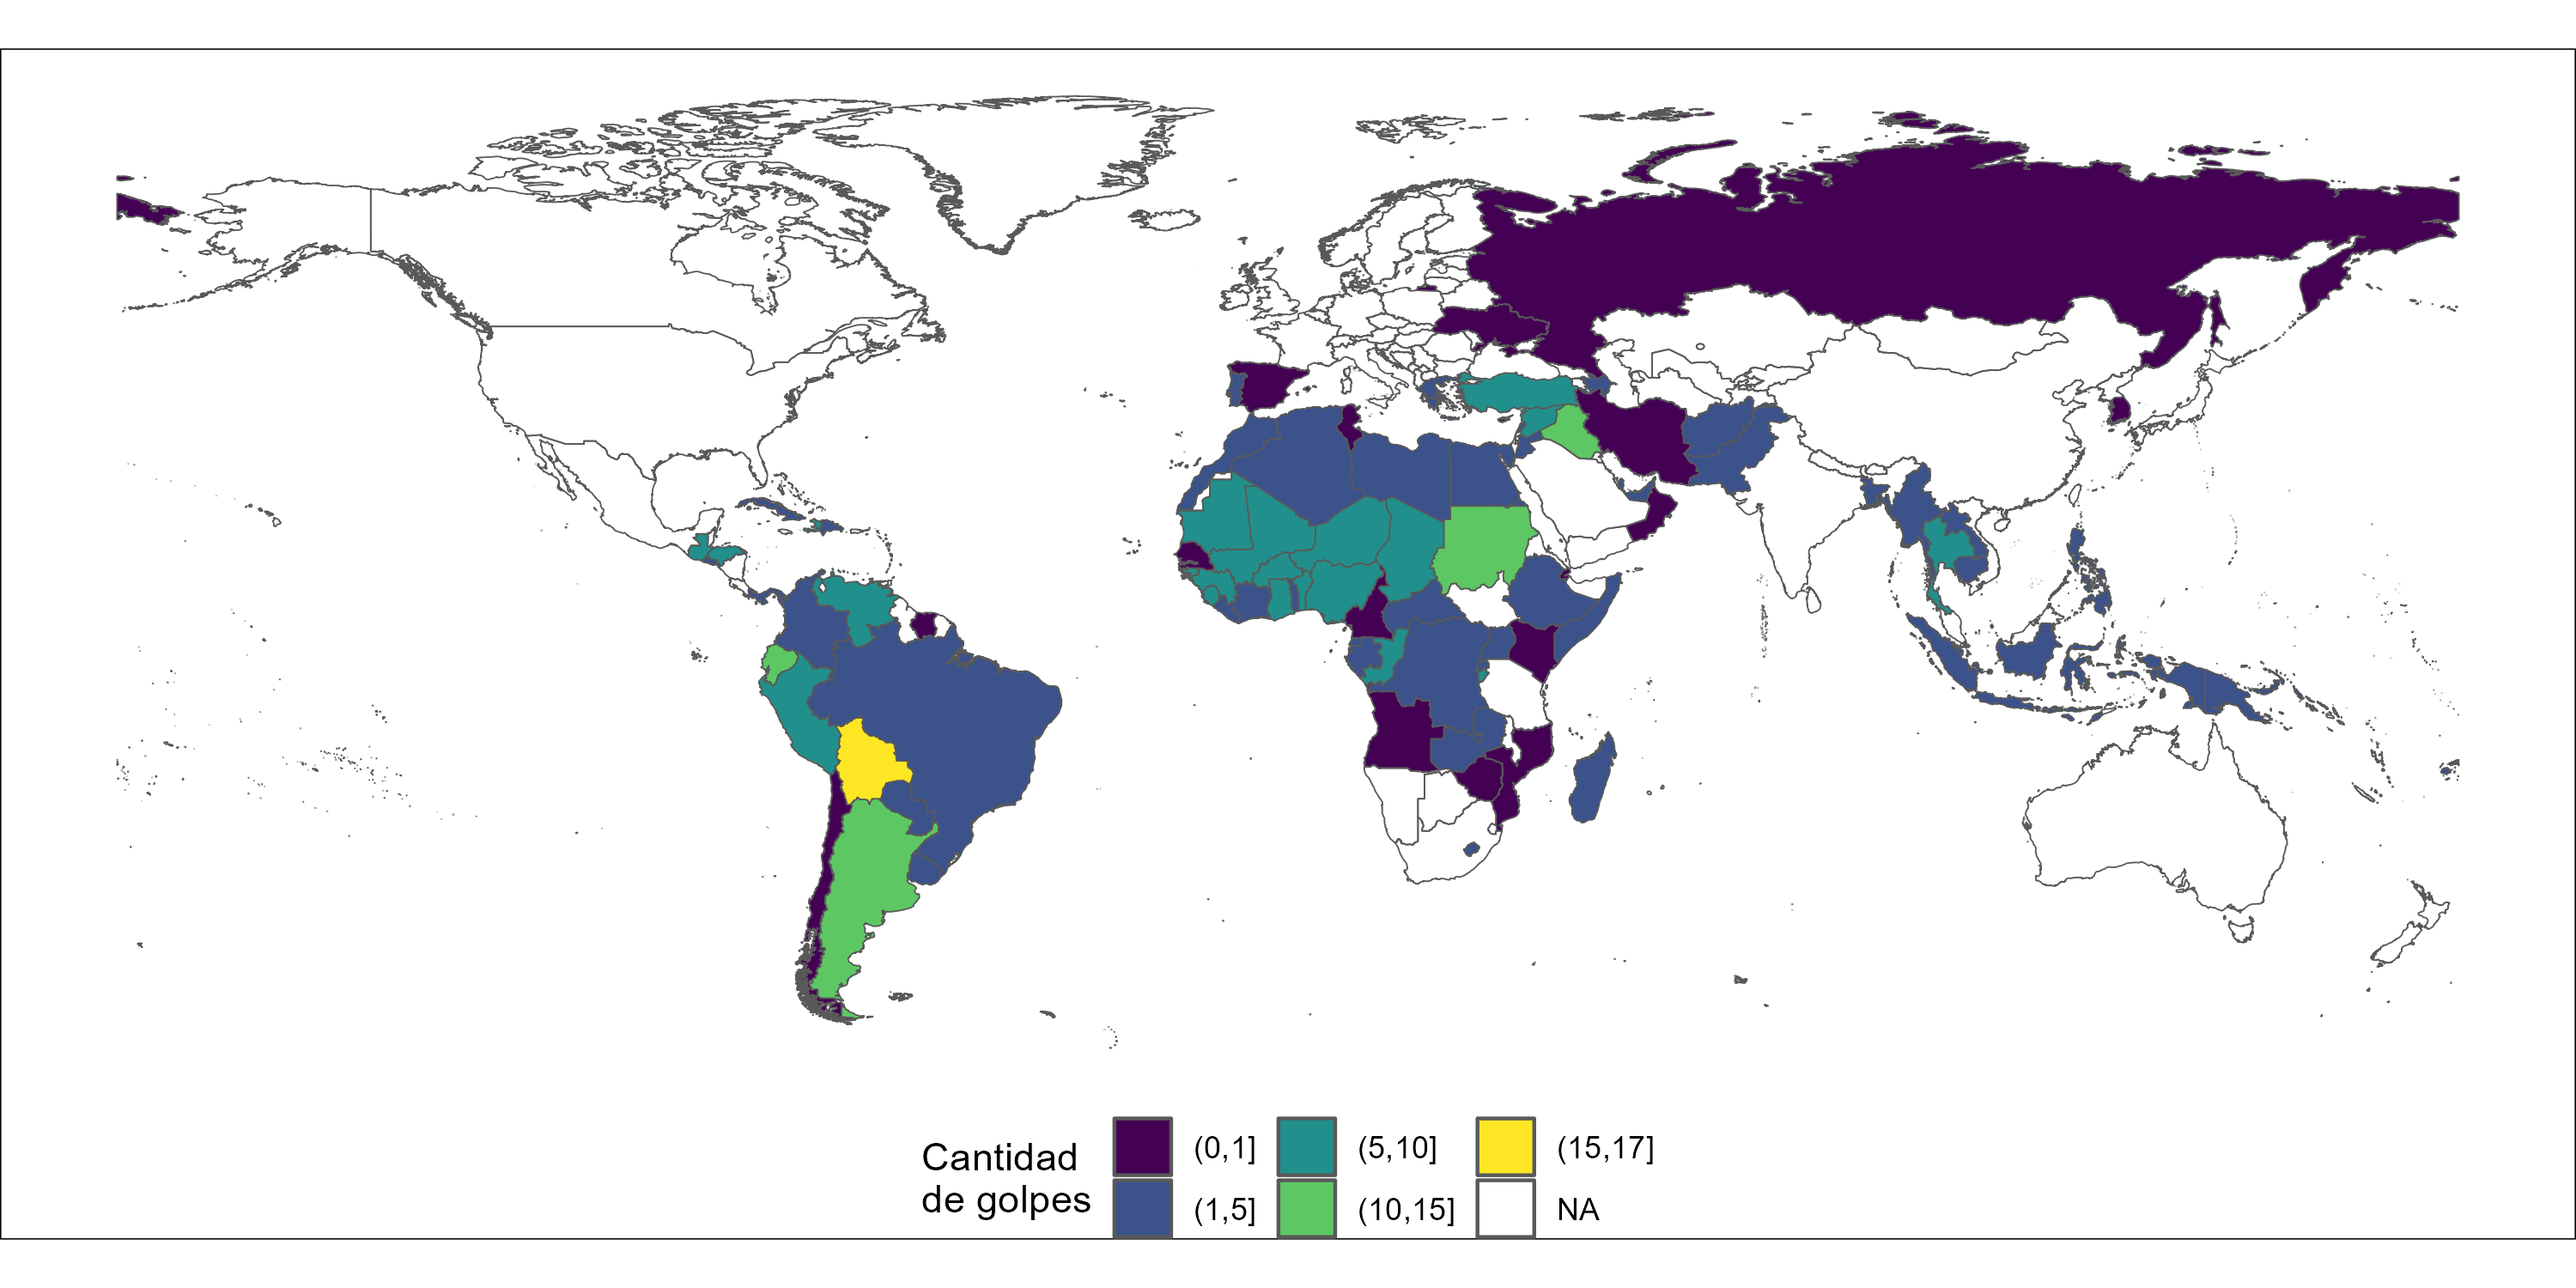
\includegraphics[width=1\textwidth]{2_golpes.png}
  \caption{Golpes de estado período (1950-2023) Fuente: \cite{Pow11} \label{fig::mapa_golpes}}
\end{figure}

Con mayor precisión, observamos que la región del Sahel se destaca con respecto a sus
vecinos africanos. Los países en donde más golpes de estado se han producido son
Bolivia (17), Sudán (14), Argentina (13), Ecuador (11), Iraq (11), Siria(11), 
Guatemala (10) y Tailandia (10).

Desagregando por década se observan algunos cambios, así como la persistencia en 
algunas regiones. La región del Sahel y varias naciones circundantes fueron 
persistentemente afectadas por golpes de estado desde los años 60. En América del 
Sur, en cambio, la presencia casi total de situaciones golpistas en la región se 
fue acotando a partir de los años 80 hasta finalmente desaparecer en el siglo 
xxi. Para observar con más detalle y discriminado por años y países se puede ver 
la figura \ref{fig:golpes_anios}.

\begin{figure}[H]
  \centering  
  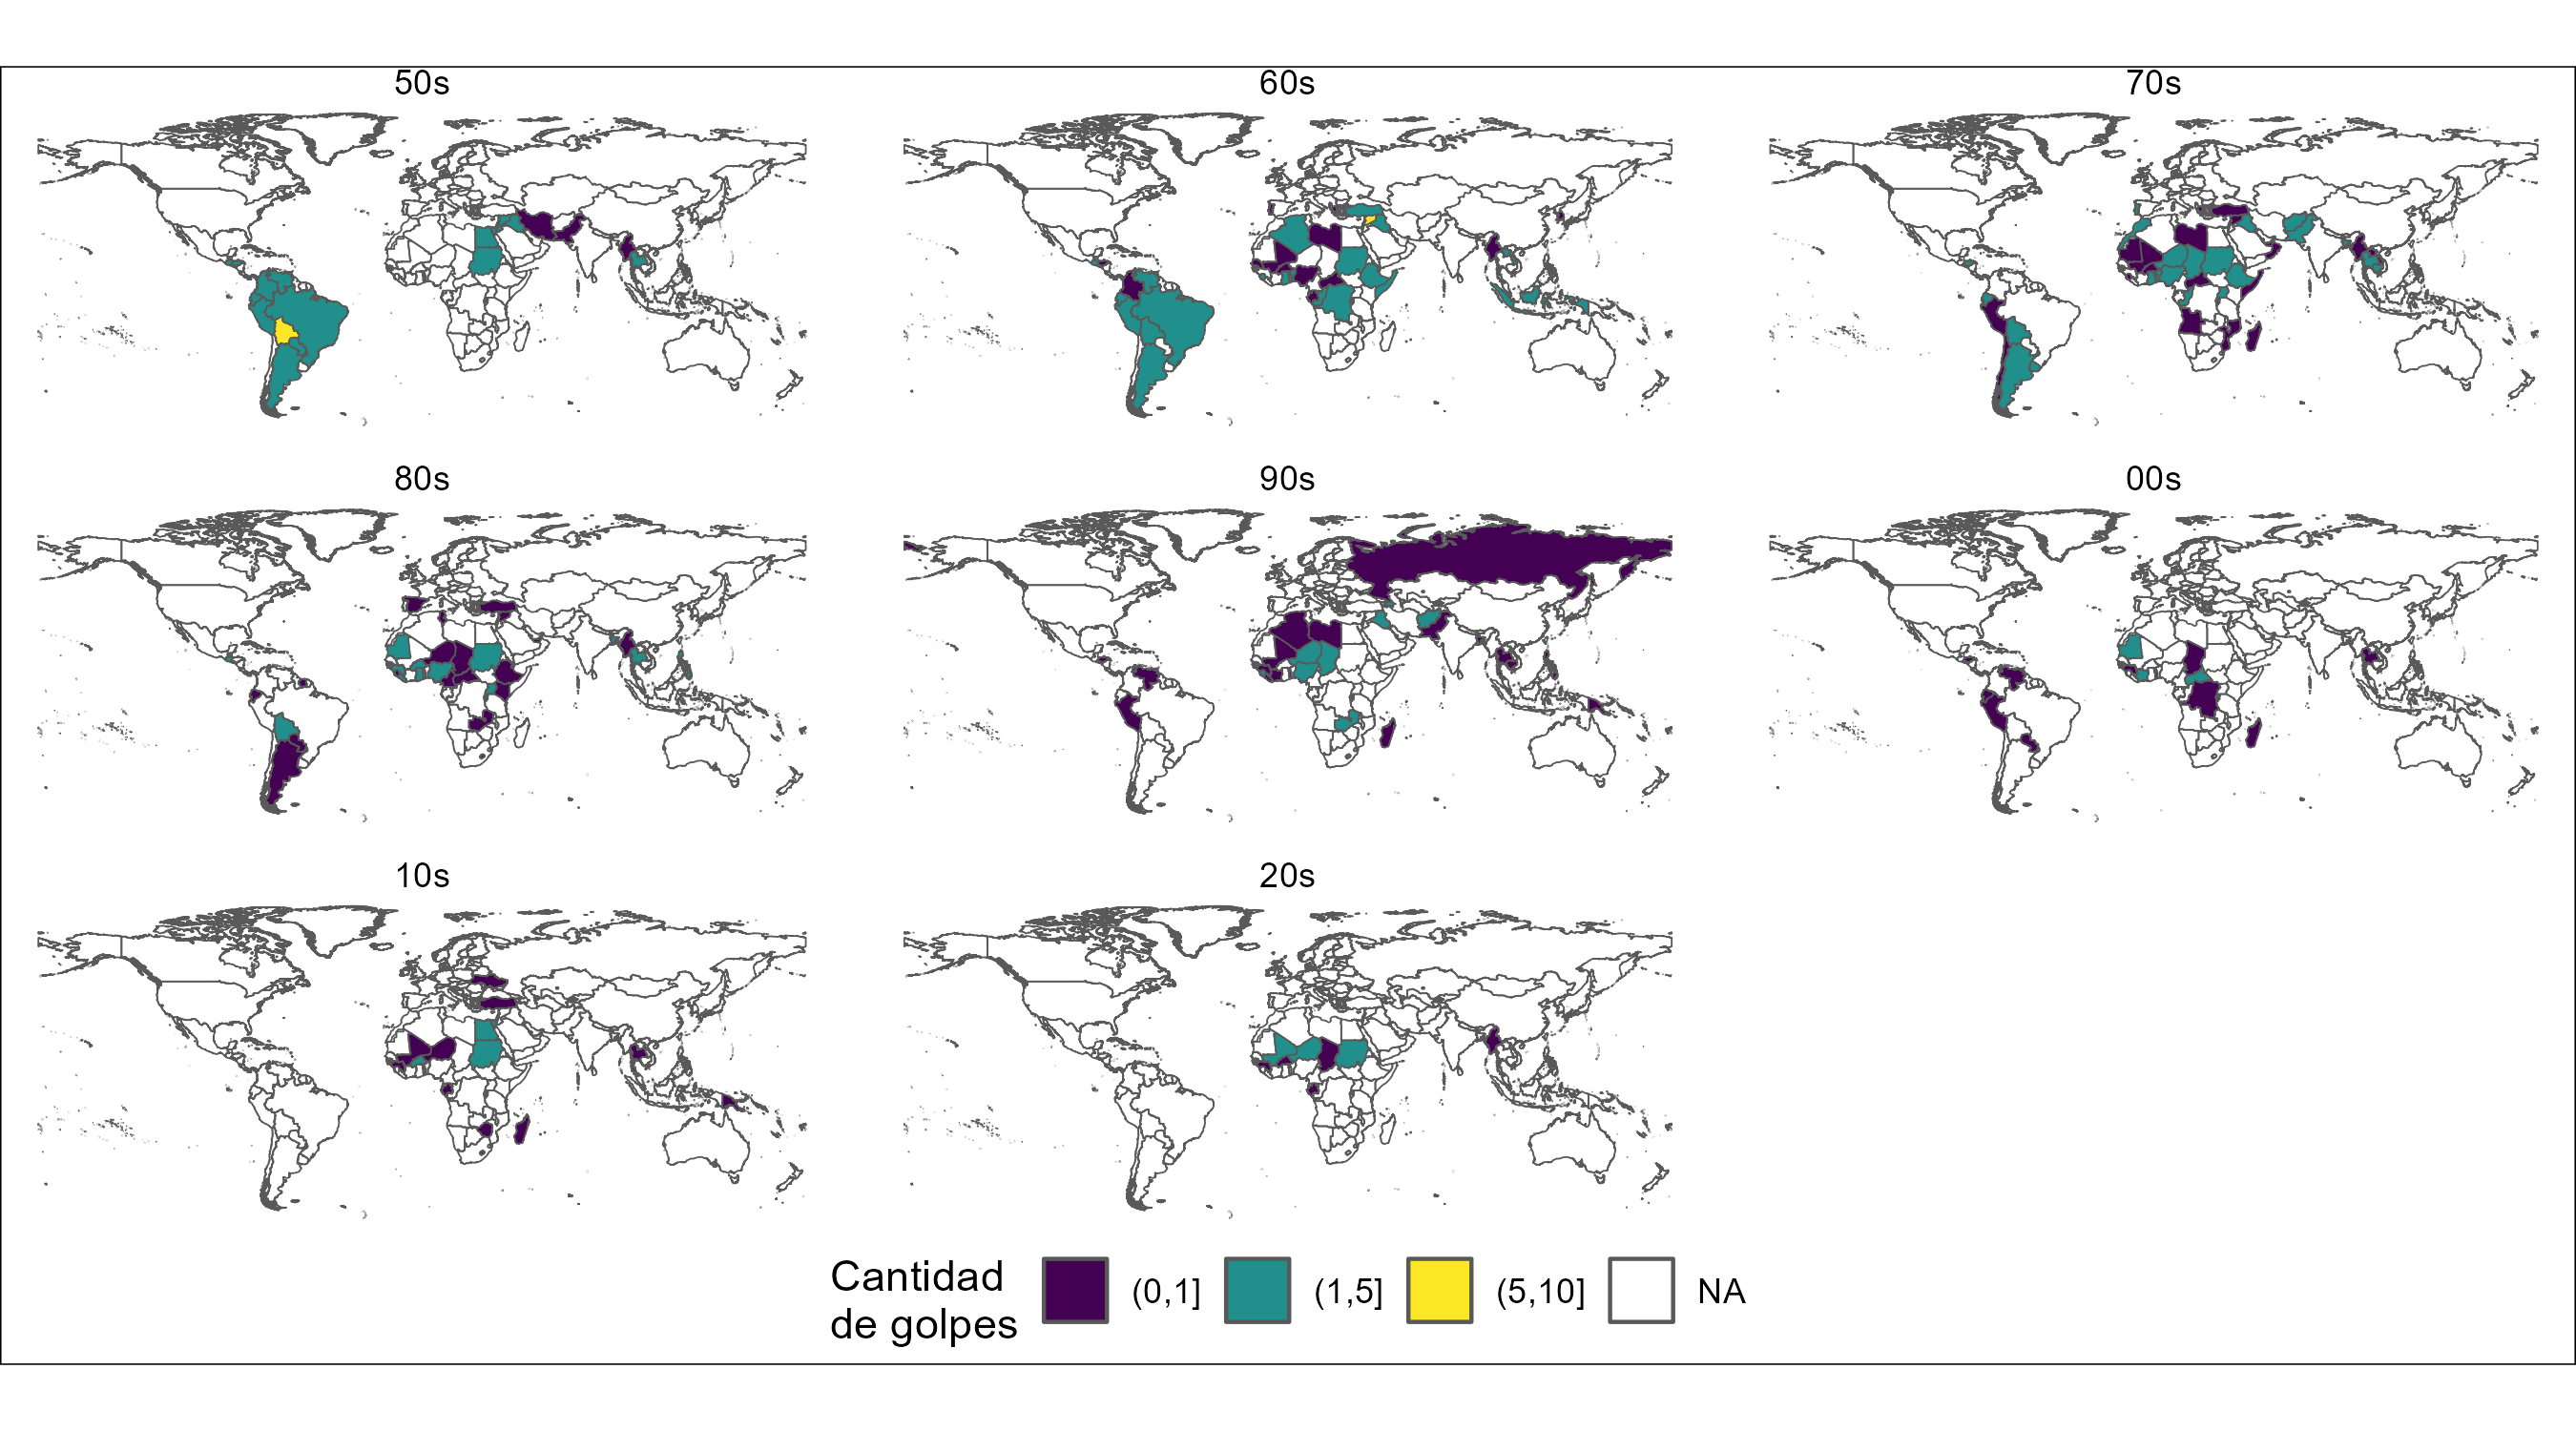
\includegraphics[width=1\textwidth]{3_golpes_decadas.png}
  \caption{Conteo de golpes por década Fuente:\cite{Pow11} \label{fig:golpes_decadas}}
\end{figure}

\section{Resultados y discusión}

\subsection{Performance de los modelos}
En primer lugar, se ralizó la optimización bayesiana de ambos modelos según lo indicado
en la metodología. En el caso de XGBoost se pudo realizar las 100 iteraciones sin mayores
inconvenientes, tomando los valores óptimos de hiperparámetros para el entrenamiento 
final. Con respecto a Random Forest, en cambio, se alcanzaron 53 iteraciones, debido a que cada
iteración consumía una gran cantidad de tiempo (en promedio una hora) y no se observaban
mejoras significativas en el AUC. De las iteraciones generadas, se tomó los 
hiperparámetros del segundo mejor AUC, puesto que la diferencia con el ganador en el score 
era insignificante, pero el tiempo de cómputo era menos de la mitad.

Una vez seleccionado los mejores hiperparámetros, se procede a entrenar los modelos en el
conjunto de entrenamiento final, el cual abarca los registros desde 1950 hasta 2019; así
como a evaluar el desempeño del mismo en los años 2020, 2021 y 2022 para emular el trabajo
realizado por el FMI.

Es importante destacar que existen dos enfoques para evaluar el modelo en los años de
testeo: por un lado se pueden evaluar todos los años en su conjunto utilizando como datos
de entrenamiento los registros hasta el año anterior del primer año de validación. Una
opción alternativa es ir entrenando el modelo hasta el año anterior al de validación para
cada año individualmente, de manera de poder utilizar todos los años anteriores y no 
perder performance. Para este trabajo utilizamos el primer enfoque, es decir que entrenamos los 
modelos hasta 2019 y los evaluamos en todos los años de evaluación a la vez, de manera de
aprehender de manera geenral la importancia de cada variable en la predicción de la
variable objetivo.

En el cuadro \ref{tab:performance} observamos el desempeño de los modelos en los años
de testeo. Por un lado figura el AUC individual de cada año por separado y por el otro
observamos el AUC acumulada es decir, evaluando en ese año junto con los anteriores.

\begin{table}[H]
  \centering
    \begin{tabular}{lcccc}
      \toprule
      & \multicolumn{2}{c}{XGBoost} & \multicolumn{2}{c}{Random Forest} \\
      Año  & AUC      & AUC      & AUC      & AUC  \\
           &          & acumulada&          & acumulada \\
      \midrule
      2020 & 1.000000 & 1.000000 & 1.000000 & 1.000000 \\
      2021 & 0.750000 & 0.785714 & 0.830443 & 0.855718 \\
      2022 & 0.666667 & 0.750000 & 0.666667 & 0.799051 \\
      \bottomrule
    \end{tabular}
  \caption{Área bajo la curva ROC por año puntual y acumulado (XGBoost y 
  Random Forest) \label{tab:performance}}
\end{table}

Lo primero que podemos observar es que ambos modelos logran una performance perfecta 
para el año 2020, lo cual resulta esperable ya que cuentan con información del año 
inmediatamente anterior. También esperable, la performance decae en los años siguientes, 
lo cual impacta en el valor del AUC acmulada. Lo más destacable es que Random 
Forest logra una mejor performance que XGBoost en el resto de años, alcanzando un AUC de 
casi 0.8 y 0.75, respectivamente. Con esta información, se tomó la decisión de continuar 
el análisis de resultados con Random Forest.

Focalizando solamente en Random Forest, y puesto que los casos negativos (527 en los 
tres años de evaluación) fueron predichos de manera perfecta, podemos aprovechar para 
visualizar los casos positivos que son apenas diez casos, tantos los verdaderos 
positivos como los falsos negativos (Cuadro \ref{tab:resultados}). En primer lugar,
podemos notar que la predicción perfecta en el año 2020 se debe a que el modelo logró
predecir correctamente el único golpe de ese año en Malí, en la región del Sahel. Después, 
en el año 2021 esta performance disminuye, al no lograr predecir los golpes de nuevo en 
Mali y en Niger, aunque si predice golpes en Sudán, Guinea y Chad. A simple vista, no parece 
haber datos geográficos o históricos que permitan establecer por qué logra predecir algunos 
golpes y en otros no,
en especial porque son países relativamente similares, de pocos años de independencia y
dentro de la misma región. Adicionalmente, en este año también logró predecir el golpe de
estado en Burma/Myanmar, una nación ubicada en una región alejada de África, en el sudeste
asiático.

\begin{table}[H]
  \centering
    \begin{tabular}{rllll}
      \toprule
      Año & País & ¿Hubo golpe? & Predicción & Resultado \\
      \midrule
      2020 & Mali                  & Sí & Sí & Verdadero positivo \\
      2021 & Burma/Myanmar         & Sí & Sí & Verdadero positivo \\
      2021 & Sudan                 & Sí & Sí & Verdadero positivo \\
      2021 & Guinea                & Sí & Sí & Verdadero positivo \\
      2021 & Chad                  & Sí & Sí & Verdadero positivo \\
      2022 & Burkina Faso          & Sí & Sí & Verdadero positivo \\
      2021 & Mali                  & Sí & No & Falso negativo \\
      2021 & Niger                 & Sí & No & Falso negativo \\
      2022 & Guinea-Bissau         & Sí & No & Falso negativo \\
      2022 & Sao Tome and Principe & Sí & No & Falso negativo \\
      \bottomrule
    \end{tabular}
  \caption{Falsos negativos y verdaderos positivos (Random Forest) \label{tab:resultados}}
\end{table}

Finalmente, el año 2022 expone la peor performance del modelo: si bien logra predecir
un golpe de estado en Burkina Faso, falla al predecir golpes en Guinea-Bissau y Sao Tome
y Principe, todos países en la misma región del continente africano. De manera general, 
podemos asociar esta baja en la performance a que el modelo deja de contar con
información del año inmediatamente anterior al del conjunto de evaluación.

\subsection{Análisis de variables}
A continuación, pasaremos a evaluar la relevancia de las distintas variables del dataset
para la predicción del modelo. De esa manera, podremos extraer elementos para determinar
o reforzar los posibles causales de un golpe de estado en un territorio determinado. En 
primer lugar, utilizaremos la importancia de las variables según Random Forest, la cual
se puede observar en la figura \ref{fig:feat_imp} (los nombres de las variables fueron
traducidas y resumidas del libro de códigos de la base de datos para una vista amigable.
Se puede verificar el nombre codificado y original de las variables en la tabla \ref{tab:vars}). 

Las barras indican el porcentaje de
importancia de las 10 variables con mayor peso. En total, estas diez variables representan
alrededor del 50\% de la importancia. En general, todas las variables están relacionadas 
con la forma de gobierno, con la influencia de las fuerzas armadas en el mismo o con la 
misma variable objetivo en años anteriores.
Entre el segundo y el cuarto lugar figuran variables
que reflejan muy evidentemente una relación con la presencia de golpes de estado, como 
tener la legislatura cerrada o abortada o que el ejecutivo no sea más electo. El dato más
interesante a destacar es que la variable con mayor importancia es la cantidad de días desde que
comenzó el régimen. Se puede inferir de esto último que un régimen joven es más inestable y, por
lo tanto, propensa a sufrir un nuevo cambio de régien mediante un golpe.

\begin{figure}[H]
  \centering  
  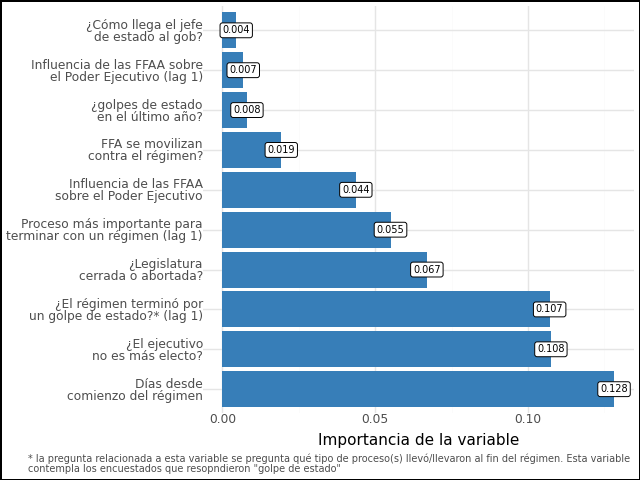
\includegraphics[width=1\textwidth]{8_feature_importance.png}
  \caption{Importancia de las variables para predicción 2020-2022 (Random Forest) \label{fig:feat_imp}}
\end{figure}

Ahora incorporaremos los Shapley Values para identificar variables importantes a la hora
de predecir la presencia de golpes de Estado, como se expone en la figura \ref{fig:shapley}.
En el eje Y figuran las primeras 11 variables con mayor valor de Shapley y en el eje X figura
el valor Shapley, visualizando la distribución de los casos en forma de violín y los outliers 
como puntos. Finalmente, el color de los violines y de los puntos indica el valor de la 
variable en cuestión.

\begin{figure}[H]
  \centering
  
\includegraphics[width=1\textwidth]{7_shapley_values.png}
  \caption{Shapley values para predicción 2020-2022 (Random Forest)\label{fig:shapley}}
\end{figure}

Si bien en este gráfico algunas variables figuran también en el gráfico de la importancia
de las variables, podemos destacar algunas diferencias. Primero, figura la enseñanza de 
valores políticos en la escuela, en cuyo valores nulos tienen alto valor Shapley. También 
destacan los datos nulos en el poder relativo entre miembros electos y no electos a nivel 
regional, en su misma versión hace 10 años (lag 10) y en la presencia de violencia durante 
el período electoral.

Para comprender qué significan estos datos nulos, es de utilidad recurrir al libro de 
códigds de la base de datos. Por ejemplo, un valor faltante en el poder relativo entre 
oficiales electos y no electos significa que todos o casi todos de los funcionarios 
electos son subordinados de algún otro poder que no surgió de las urnas (a nivel
regional).

Otros temas a tratar en los resultados en la próxima entrega:
- Valores Shapley en cada año individual y/o en cada país
- Análisis histórico de las variables destacadas

\subsection{Discusiones}
- Vinculación de resultados con estado del arte y marco teórico

- Comparación de performance y de variables importantes con el artículo del FMI

- Limitaciones 

\section{Conclusiones}
- Resumen de los hallazgos principales

- Conclusiones generales y su relación con los objetivos del trabajo

- Recomendaciones para futuros trabajos


\section{Anexo}
\subsection{Código}
La totalidad del código y entregas en latex y PDF se encuentran en un repositorio abierto de
Github de José Saint Germain (\href{https://github.com/josesg998/esp_data_mining}{Acceso al 
repositorio}). En el mismo se describe la secuencia de códigos a correr para la obtención de 
datos, la ingeniería de atributos, la optimización bayesiana, la corrida final, el análisis 
exploratorio de datos y el análisis de resultados de los algoritmos.

\subsection{Golpes}
- Breve descripción de los 10 golpes que se buscaron predecir. Su contexto histórico, político y 
social.
\subsection{Gráficos y tablas adicionales}
\begin{figure}[H]
  \centering  
  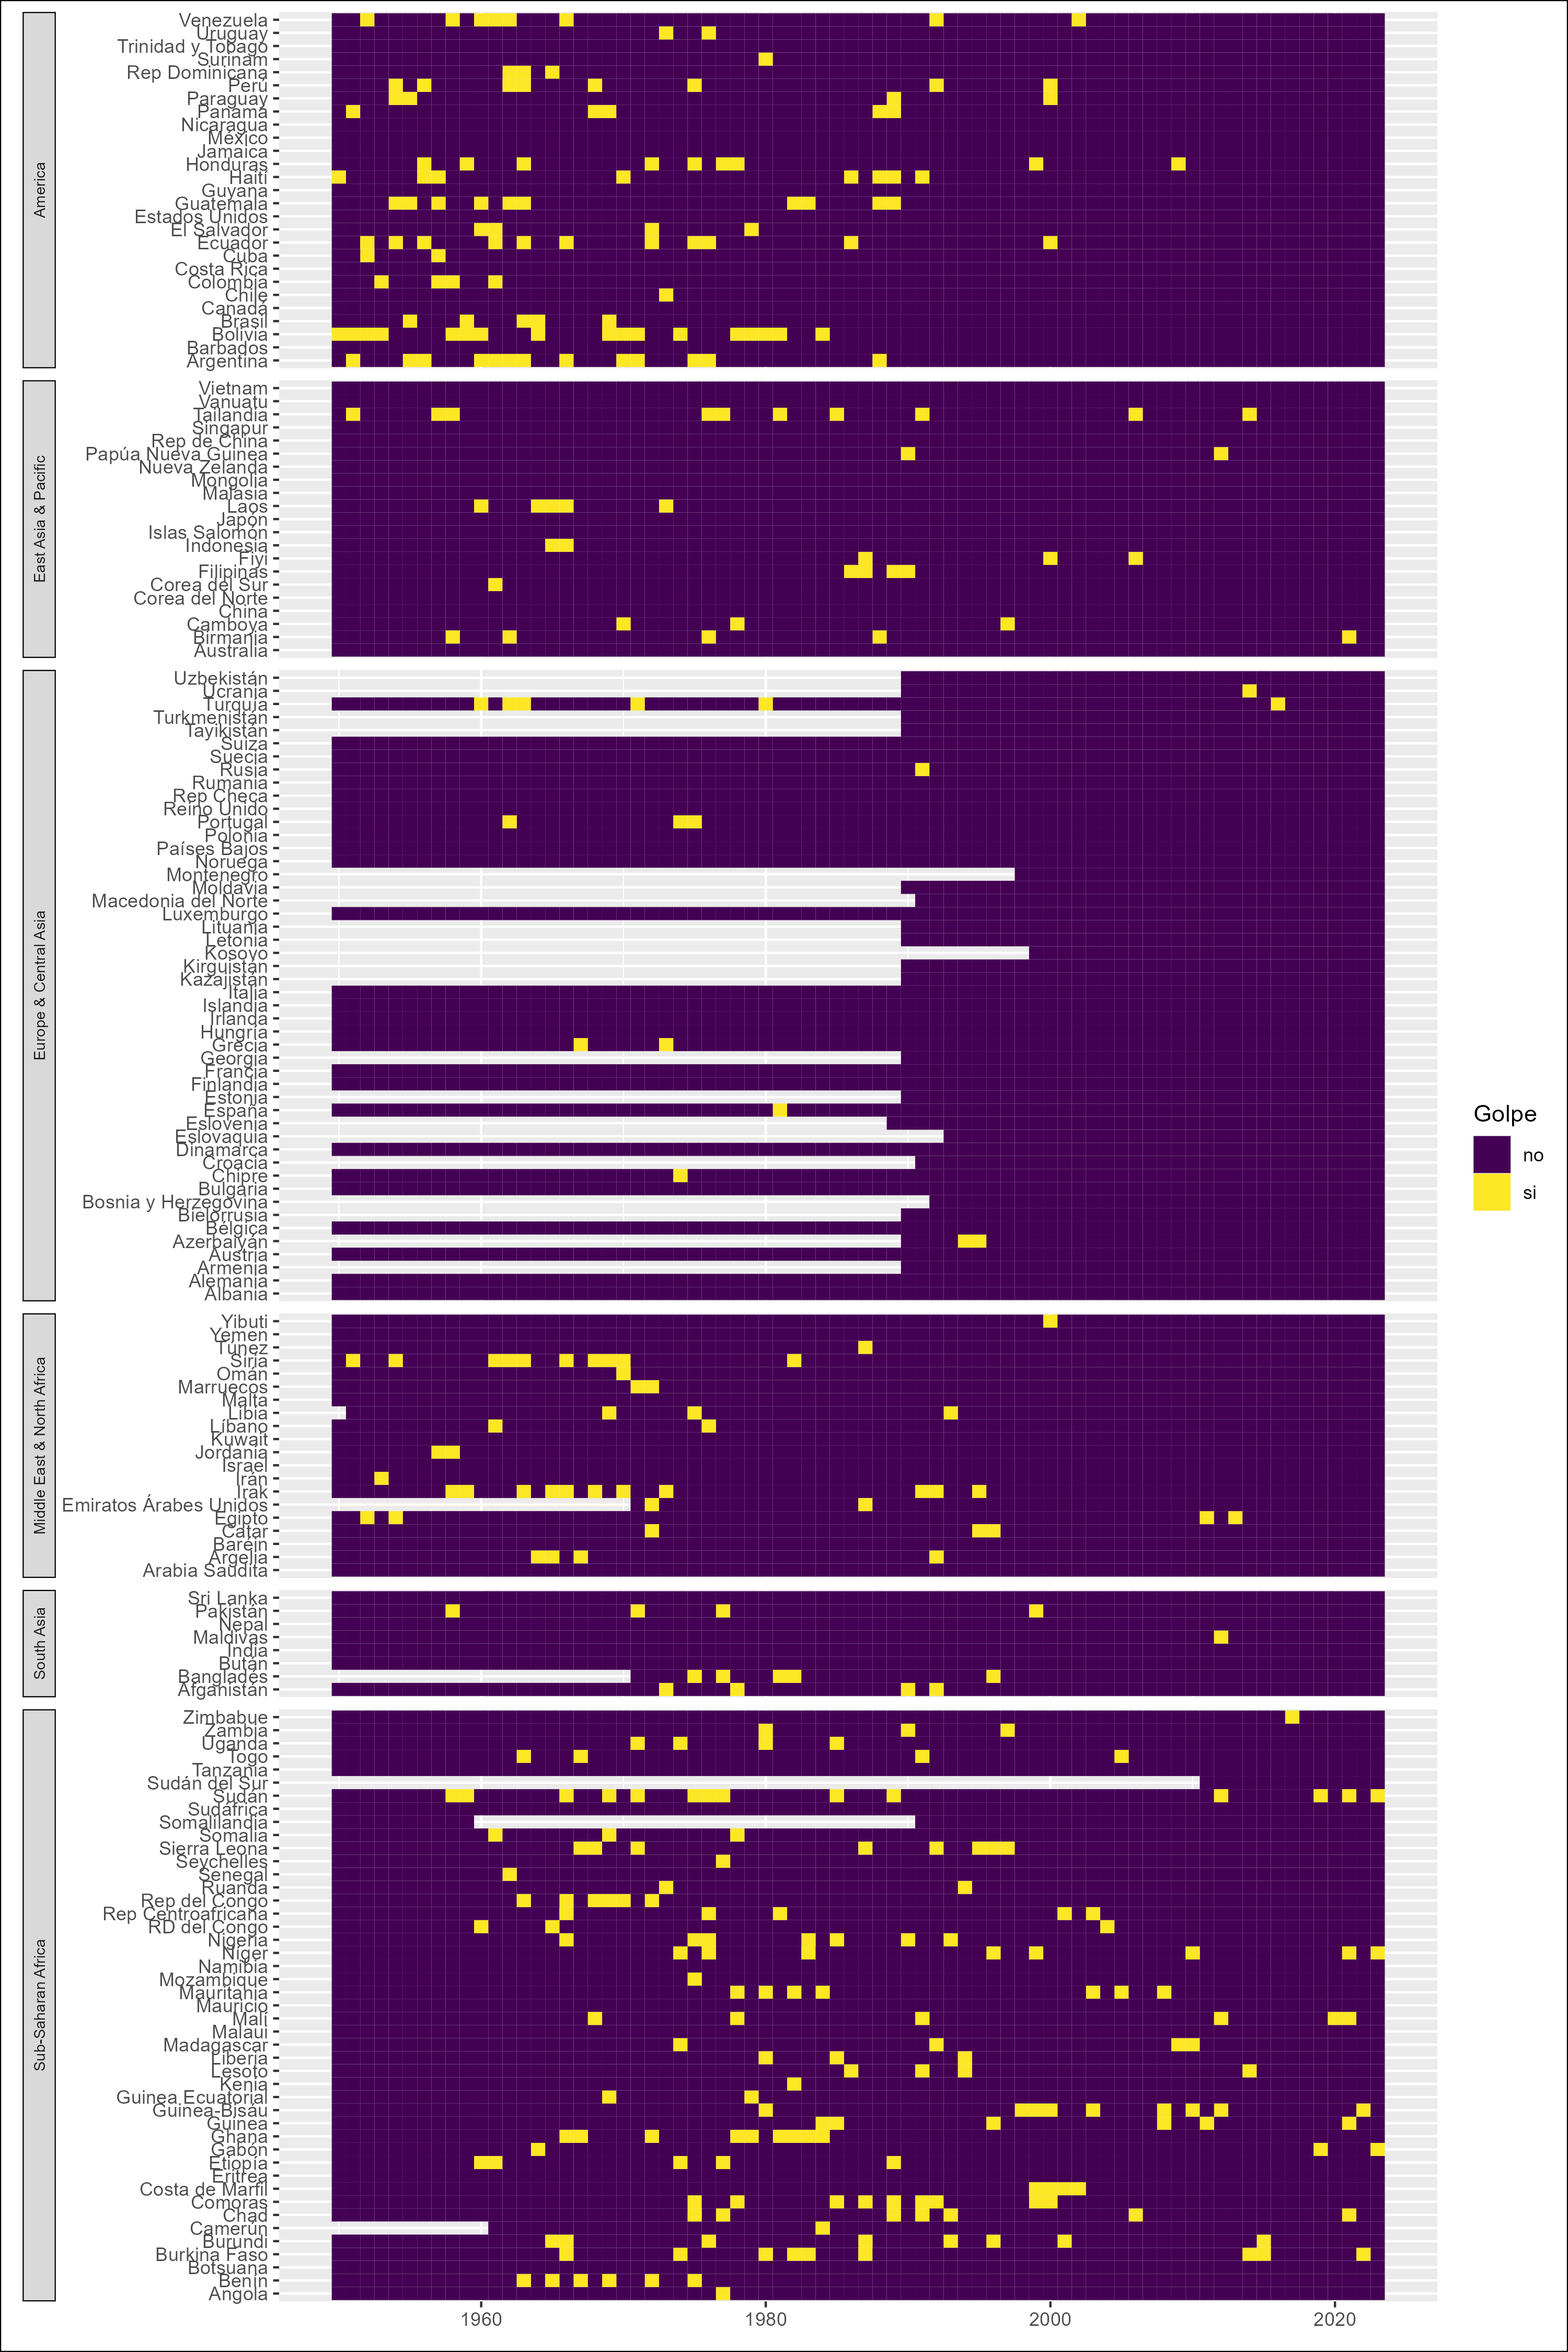
\includegraphics[width=1\textwidth]{4_golpes_anios.png}
  \caption{Conteo de golpes por año y región (\cite{Pow11})\label{fig:golpes_anios}}
\end{figure}

\begin{table}[H]
  \begin{tabular}{ll}
    \toprule
    Variable                  & Descripción \\
    \midrule
    coup\_lag\_1              & ¿golpes de estado en el último año? \\
    v2expathhs                & ¿Cómo llega el jefe de estado al gob? \\
    v2regdur                  & Días desde comienzo del régimen \\
    v2regoppgroupsact\_5      & FFA se movilizan contra el régimen? \\
    v2elrgpwr\_lag\_5         & Poder relativo entre miembros electos y no electos a nivel regional (lag 5) \\
    v2edpoledprim\_lag\_5     & ¿Se enseña en la primaria contenidos con valores políticos? (lag 5) \\
    v2elpeace                 & Violencia durante período electoral \\
    v2x\_ex\_military         & Influencia de las FFAA sobre  el Poder Ejecutivo \\
    v2x\_ex\_military\_lag\_1 & Influencia de las FFAA sobre el Poder Ejecutivo (lag 1) \\
    v2elrgpwr\_lag\_10        & Poder relativo entre miembros electos y no electos a nivel regional (lag 10) \\
    v2x\_hosinter             & ¿El ejecutivo no es más electo? \\
    v2regendtypems\_0\_lag\_1 & ¿El régimen terminó por un golpe de estado? (lag 1) \\
    v2xlg\_leginter           & ¿Legislatura cerrada o abortada? \\
    v2regendtype\_lag\_1      & Proceso más importante para terminar con un régimen (lag 1) \\
    coup\_lag\_1              & ¿Golpes de estado en el último año? \\
    \bottomrule 
    \end{tabular}
  \caption{Nombre original de variables y su descripción \label{tab:vars}}
\end{table}

\printbibliography

\end{document}